\documentclass[UTF8,a4paper,11pt]{ctexart}

\usepackage[a4paper,margin=2.25cm]{geometry}
\usepackage{amsmath,amssymb,mathtools}
\usepackage{booktabs}
\usepackage{graphicx}
\usepackage{caption}
\usepackage{subcaption}
\usepackage{tabularx}
\usepackage{array}
\usepackage{multirow}
\usepackage{enumitem}
\usepackage{microtype}
\usepackage{setspace}
\usepackage[hidelinks]{hyperref}

\graphicspath{{figures/}}
\setstretch{1.16}
\setlength{\parindent}{2em}
\setlength{\parskip}{0.18em}
\emergencystretch=2em
\captionsetup{font=small,labelfont=bf,labelsep=quad}
\renewcommand{\arraystretch}{1.15}
\newcolumntype{Y}{>{\raggedright\arraybackslash}X}

\title{\heiti 主流大语言模型综合性能评价与场景化选择\\基于缺失感知 Bradley--Terry 与 CES 的数学建模}
\author{}
\date{}

\begin{document}
\maketitle

\begin{abstract}
针对题目提出的主流大语言模型综合性能评价与场景选择问题，本文构建“基础能力识别—场景适配—预算决策”的递进模型。问题一面向 10 个模型、21 个 Exact Setting 和 14 个 Benchmark Family，针对公开评测量纲不一、信息冗余和成绩缺失等困难，采用缺失感知 Spearman、Family 平衡成对比较和正则化 Bradley--Terry 估计复杂推理、知识与事实可靠性、长上下文、代码与软件工程、多模态五维能力，并以信息量、非冗余度和稳定性确定综合权重。有效观测覆盖率为 $164/210=78.1\%$，Ranking A 的点估计中 GPT-5.6 Sol、Claude Fable 5 和 Kimi K3 分列前三。问题二针对综合排序不能表达任务差异的问题，以 KL 最小信息投影确定科研、日常和代码场景权重，并用 CES 聚合描述能力互补和短板效应；结果显示科研场景由 Claude Fable 5 居首，代码场景由 Kimi K3 居首。问题三进一步考虑输入/输出 Token 工作负载成本，在成本信息完整的模型集合上构造效用--成本 Pareto 前沿和预算决策区间；代码场景的推荐节点依次为 DeepSeek-V4-Flash、DeepSeek-V4-Pro 和 Kimi K3，对应阈值为 0.01056、0.03168 和 0.10683 USD。结果表明，不存在脱离任务需求与预算约束的绝对最优模型，模型选择应依次经过基础能力识别、场景适配和预算约束三层判断。

\noindent\textbf{关键词：}大语言模型；Bradley--Terry；CES；缺失感知；Bootstrap；Pareto 前沿；成本约束
\end{abstract}

\section{问题重述}
本文围绕题目提出的主流大语言模型评价与选择问题展开。公开评测结果能够反映模型在不同任务上的表现，但各测试的量纲、覆盖范围和发布完整性并不一致；同一模型的公开成绩还可能因评测设置不同而出现缺失。因此，题目中的“综合评价”不能简单理解为把所有分数相加，而应先回答三个相互衔接的问题。

\subsection{问题一：主流模型的综合性能评价}

题目要求依据公开评测信息，对候选模型进行综合比较。其数学转译为：在模型--测试矩阵存在缺失、不同测试不可直接相加且同类测试可能重复计量的条件下，建立可比的多维能力评价体系，给出各模型的五维能力结构、综合得分和排序，并检验结论对样本与指标变化的敏感性。

问题一的输出包括复杂推理、知识与事实可靠性、长上下文、代码与软件工程、多模态五个能力维度的相对得分，以及基于正式权重的 Ranking A 综合结果。该结果回答的是“模型具有什么基础能力”，并不直接回答某一类任务中应当选择谁。

\subsection{问题二：不同任务场景下的模型选择}

综合能力排序只能给出总体评价，不能表达科研长文本分析、大众日常通用对话和计算机代码开发对能力组合的不同需求。题目进一步要求把模型能力与具体使用场景联系起来。其数学转译为：以问题一得到的五维能力为输入，根据题设场景需求确定能力权重，并用能够体现能力互补和短板约束的聚合函数计算场景效用。

问题二的输出是三类场景内的效用与排名。不同场景使用的能力集合和替代弹性不同，因而效用只在同一场景内比较。该结果回答的是“模型是否适合某类任务”，也解释了为什么综合排名靠前的模型在场景中可能发生名次迁移。

\subsection{问题三：成本约束下的部署决策}

即使模型在某一场景中具有较高效用，也不能据此直接作出部署选择。输入长度、输出长度、调用次数和 API 单价共同决定任务成本，且成本信息可能存在可核验性差异。题目要求在性能与成本之间进行权衡。其数学转译为：将问题二的场景效用与标准化工作负载成本联合起来，构造效用--成本 Pareto 前沿，并在不同预算上限下给出最优可行模型。

由此，三问构成递进关系：
\[
\text{公开评测信息}
\longrightarrow
\text{基础能力识别}
\longrightarrow
\text{场景适配}
\longrightarrow
\text{预算约束下的部署决策}.
\]


\section{问题分析}
\subsection{从题目要求到建模路线}

三个问题的难点不在于计算一个总分，而在于评价对象、任务需求和部署约束分别属于不同层次。若直接对公开成绩求平均，首先会混合不同测试尺度，其次会把同一 Benchmark Family 中的重复信息计算多次，最后还可能把“未公开”错误解释为“能力最低”。因此，问题一需要先处理数据语义，再建立可比的模型间关系。

问题一得到的综合排序仍不能直接用于所有任务。科研长文本分析需要在复杂推理、事实可靠性和长上下文之间形成协同；代码开发更依赖复杂推理与代码工程能力的共同支撑；日常通用对话则允许更广泛的能力组合。若采用线性加权，某一项能力的不足可以被其他高分能力完全补偿，这与存在关键短板的任务特征不符。因此，问题二采用场景权重与 CES 聚合，将能力结构转译为任务效用。

场景效用解决了适配性问题，但仍没有回答“预算允许时应该选谁”。价格本身也不是任务成本：输入/输出 Token 数量和调用次数会改变各模型的实际支出，代码任务的输出负载较高时，输出单价差异尤其容易被放大。问题三因此保留场景效用，只增加工作负载成本，并以 Pareto 前沿和预算区间表达部署选择。

\subsection{全文建模框架}

图~\ref{fig:framework}将上述逻辑归纳为三层。第一层从公开评测得到模型的基础能力；第二层把能力映射为科研、日常和代码三类任务的效用；第三层在成本和预算约束下确定可行的优选节点。图中第一层的缺失与冗余处理保证“有什么数据”不被误读，第二层的场景权重回答“任务需要什么”，第三层的 Pareto 与预算区间回答“在现实约束下选谁”。因此，三问不是三个相互独立的排名，而是由能力识别逐步走向任务决策。

\begin{figure}[htbp]
\centering
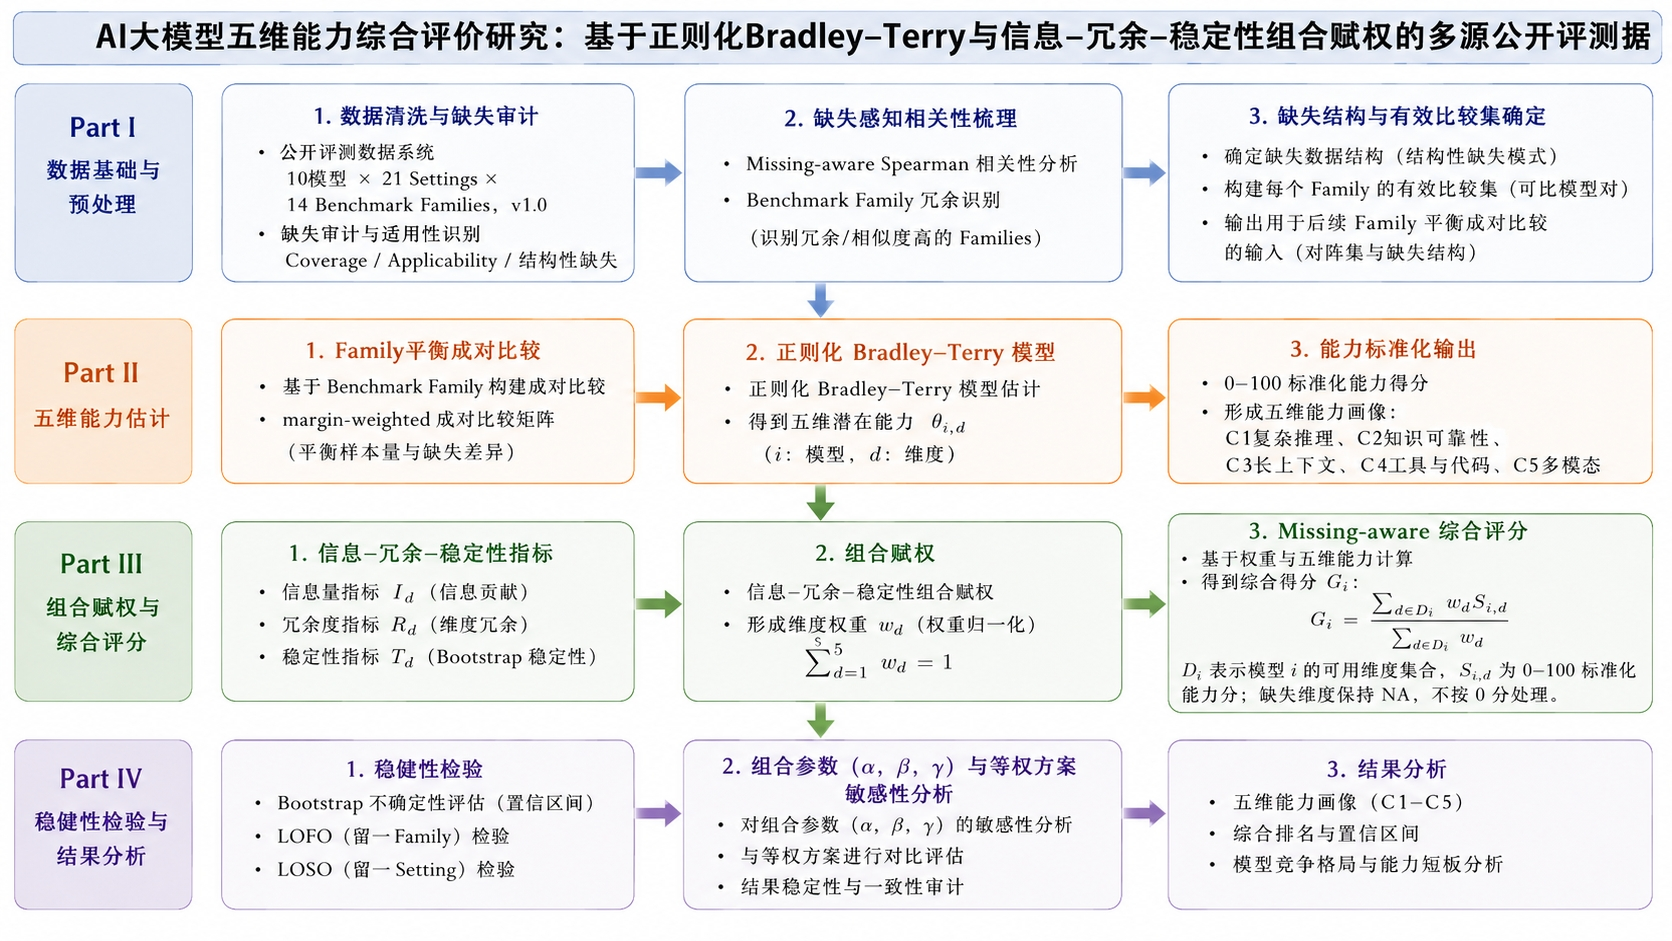
\includegraphics[width=\textwidth]{fig_framework_user.jpg}
\caption{全文建模框架。第一层统一公开评测并识别模型能力，第二层将五维能力映射为场景需求，第三层在工作负载成本和预算约束下形成部署决策。}
\label{fig:framework}
\end{figure}


\section{模型假设与符号}
\subsection{模型假设}
\begin{enumerate}[label=(\arabic*),leftmargin=2.5em]
\item 每个 Benchmark/Exact Setting 内的公开分数可以用于模型间相对比较，但不同 Benchmark/Exact Setting 的原始分数不直接相加。
\item 缺失值保持缺失。结构性能力缺位只在综合能力可用性层单独编码，不将其解释为原始 Benchmark 得分为零。
\item Benchmark Family 内部的多个 Exact Setting 可能重复表达同一能力，因此在成对比较阶段进行 Family 平衡。
\item Q2 的场景效用只用于同一场景内比较；不同场景的效用尺度不作跨场景绝对比较。
\item Q3 的工作负载是用于模型间可比性的标准化任务包，不等同于任意真实用户的平均调用量。
\item Q3 主 Pareto 分析只使用成本信息完整且人工核验通过的模型集合；价格缺失或配置账单不完整的模型不进行插补。
\end{enumerate}

\subsection{主要符号}
\begin{center}
\small
\begin{tabularx}{0.94\textwidth}{>{\raggedright\arraybackslash}p{0.18\textwidth}Y}
\toprule
符号 & 含义\\
\midrule
$i,j$ & 模型索引\\
$b$ & Benchmark/Exact Setting 索引\\
$s$ & 场景索引，取 Research、General、Coding\\
$d$ & 能力维度索引，$C_1$--$C_5$\\
$x_{ib}$ & 模型 $i$ 在 Exact Setting $b$ 上的公开分数\\
$\theta_{id}$ & 模型 $i$ 在能力维度 $d$ 上的 BT 潜在能力\\
$S_{id}$ & 由 $\theta_{id}$ 转换得到的 0--100 维度得分\\
$w_d$ & Q1 综合评价权重；$w_d(s)$ 为 Q2 场景权重\\
$U_i^{(s)}$ & 模型 $i$ 在场景 $s$ 下的 CES 效用\\
$C_i^{(s)}$ & 模型 $i$ 在场景 $s$ 下的标准任务成本\\
$N_s,L_{\mathrm{in}}^{(s)},L_{\mathrm{out}}^{(s)}$ & 场景调用次数、输入 Token 数和输出 Token 数\\
\bottomrule
\end{tabularx}
\end{center}


\section{问题一：缺失感知的五维能力评价}
\subsection{为什么问题一需要缺失感知的比较体系}

题目要求依据公开评测结果评价候选模型，但不同 Benchmark 的量纲、难度和测试协议并不相同，模型公开成绩也不是完整矩阵。当前数据包含 10 个模型、21 个 Exact Setting 和 14 个 Benchmark Family，理论上有 \(210\) 个模型--设置组合，其中只有 \(164\) 个有效观测，覆盖率为
\[
\eta=\frac{164}{10\times21}=0.780952.
\]
若采用完整案例删除，将同时损失模型和 Benchmark 信息；若把缺失填为 0，又会把“未公开”或“不适用”误解释为“能力最低”。因此，本问先保留缺失语义，再在同一测试设置内建立模型间可比的相对关系。

\begin{figure}[htbp]
\centering
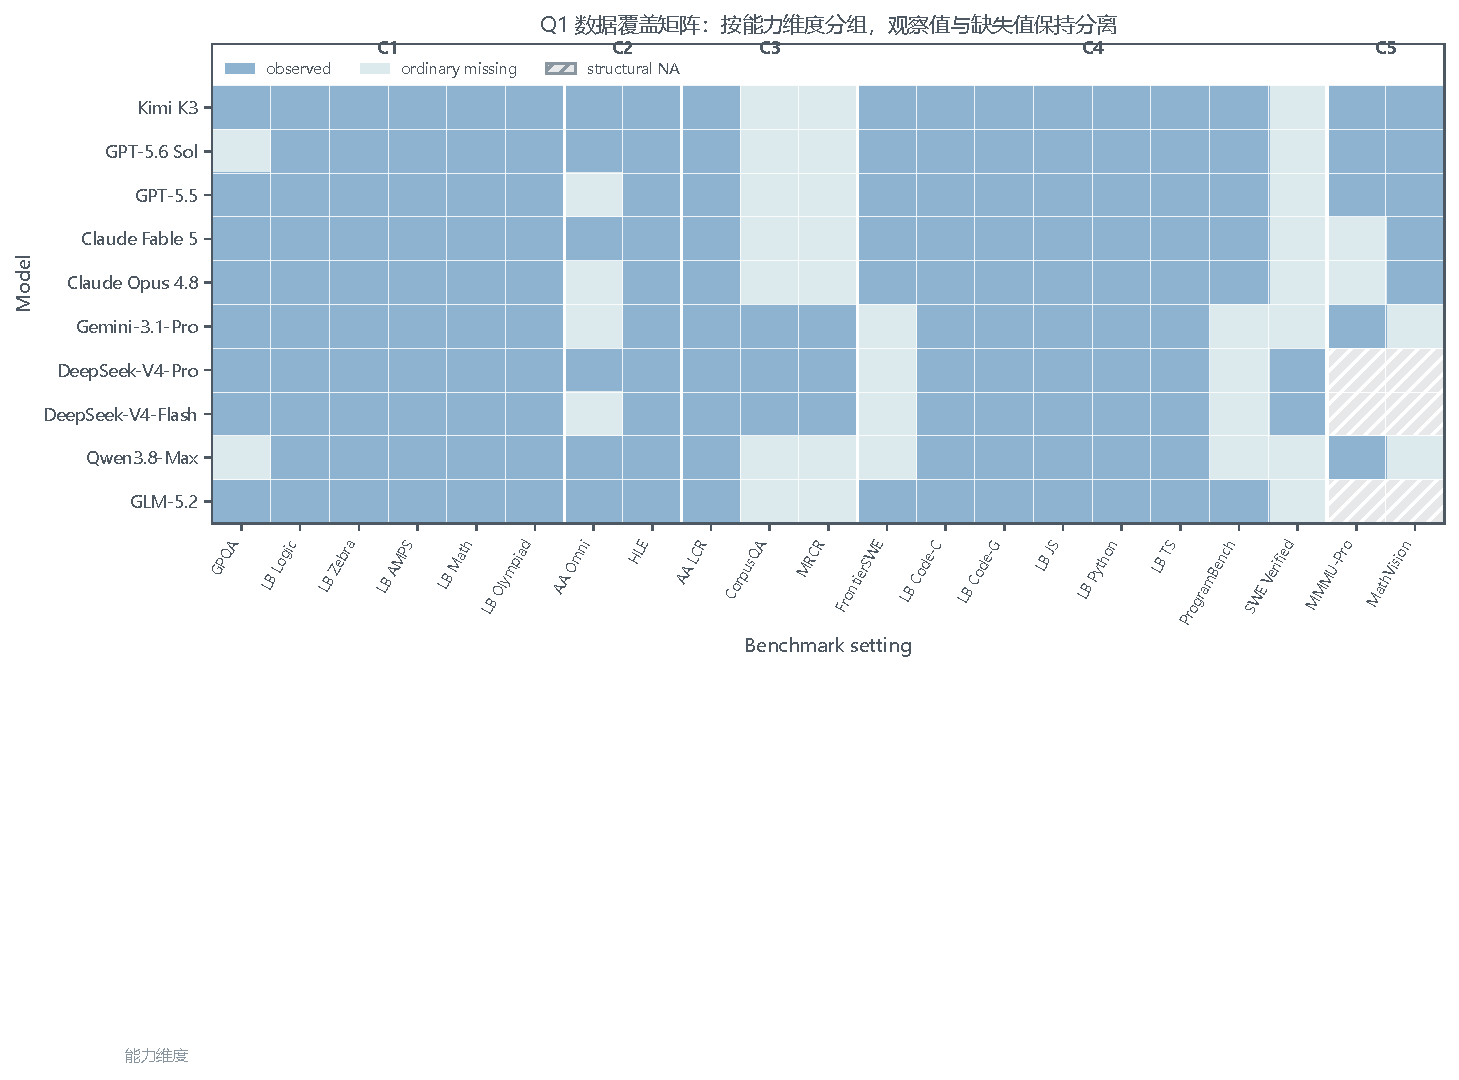
\includegraphics[width=\textwidth]{fig_q1_coverage.pdf}
\caption{Q1 数据覆盖矩阵。横轴使用简短 Benchmark 标签，上方按 \(C_1\)--\(C_5\) 分组；深色为 observed，浅色为 ordinary missing，带纹理的浅灰单元格仅表示有适用性审计依据的 structural NA。}
\label{fig:q1coverage}
\end{figure}

图~\ref{fig:q1coverage}表明，缺失并非均匀分布在所有能力维度上。C5 的部分模型由于不具备题设定义下的原生多模态能力而出现结构性缺位，不能与普通未公开成绩混为一谈。该数据结构决定了问题一必须采用缺失感知的评价方法。

\subsection{缺失感知相关性与 Benchmark Family 平衡}

不同 Benchmark 可能重复反映相近能力。若直接把所有 Exact Setting 等权相加，一个包含更多设置的 Family 会获得隐含的重复权重。为此，对两个设置 \(a,b\) 在共同有效模型集合
\[
I_{ab}=\{i:x_{ia}\ \text{和}\ x_{ib}\ \text{均有效}\}
\]
上计算 Spearman 秩相关 \(\rho_{ab}\)，并同时记录共同样本数 \(N_{ab}=|I_{ab}|\)。图~\ref{fig:q1spearman}的下三角表示秩相关，上三角给出 Common-N。

\begin{figure}[htbp]
\centering
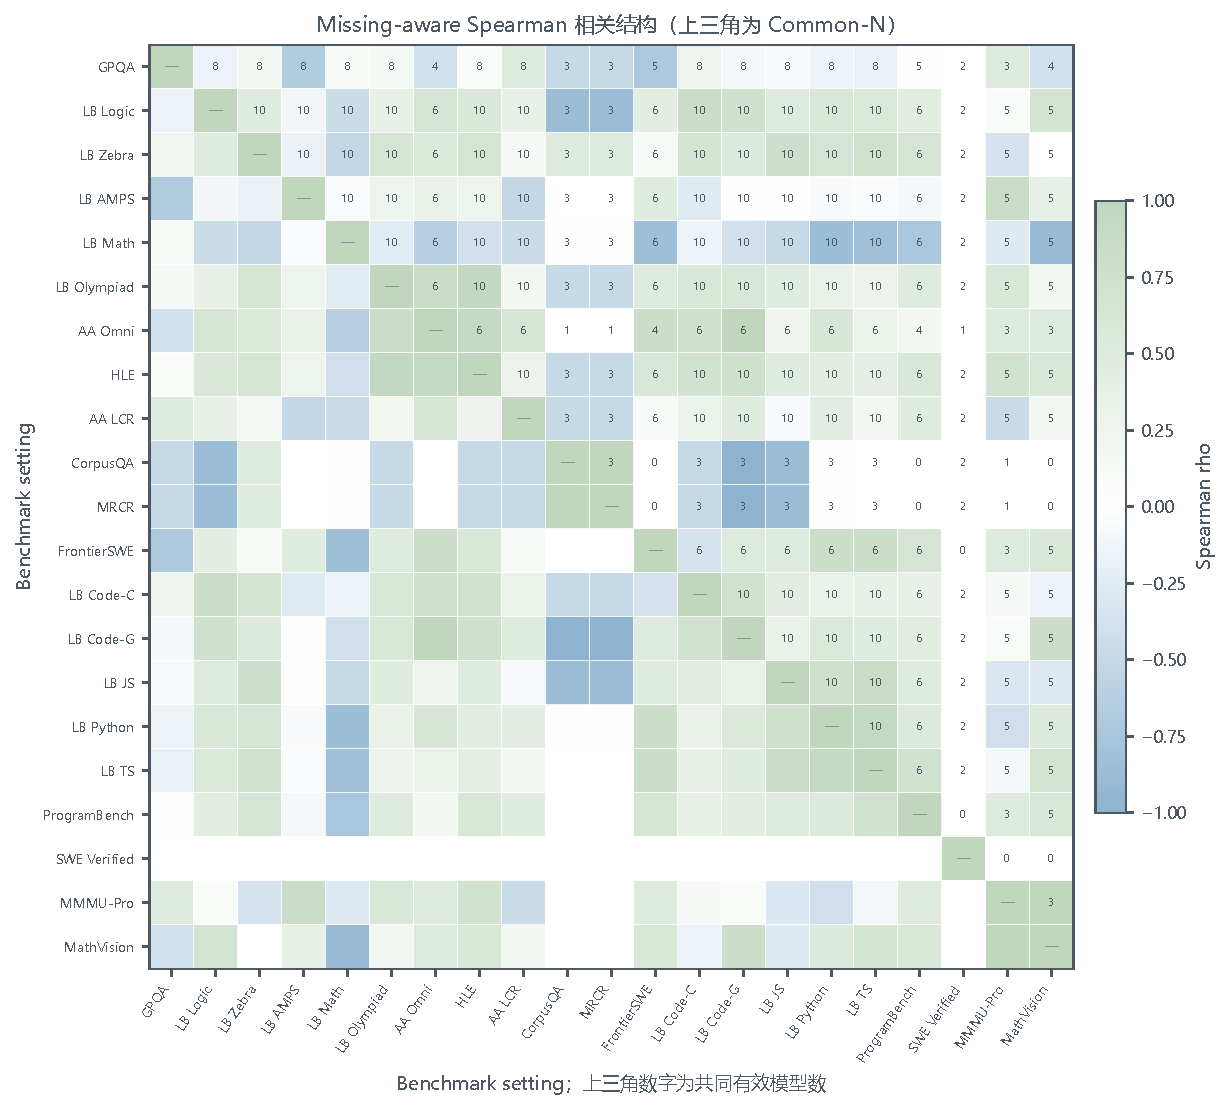
\includegraphics[width=0.86\textwidth]{fig_q1_spearman.pdf}
\caption{缺失感知 Spearman 相关矩阵。下三角颜色表示 \(\rho_{ab}\)，上三角数字表示共同有效模型数 Common-N；较小的 Common-N 不作复杂纹理叠加，而在正文中单独解释。}
\label{fig:q1spearman}
\end{figure}

高 \(|\rho|\) 只说明潜在信息冗余，不能自动推出应删除某个 Benchmark。若 Common-N 较小，相关性可能不稳定；若某设置承担不同模型群体之间的桥接作用，删除后还可能使比较网络断开。因此，本文只将相关分析作为冗余证据，并结合 Family 平衡和后续 LOFO 检验决定其影响。

\subsection{正则化 Bradley--Terry 能力估计}

不同测试的原始分数不宜直接相加，但同一 Exact Setting 内的模型相对优劣仍具有可比性。设模型 \(i,j\) 在设置 \(b\) 上的相对结果为
\[
y_{ijb}=
\begin{cases}
1,&x_{ib}>x_{jb},\\
0.5,&x_{ib}=x_{jb},\\
0,&x_{ib}<x_{jb}.
\end{cases}
\]
任一模型缺失该设置时不构造成对关系。为保留领先幅度，按同一设置内的相对差值构造 margin 权重，再在能力维度内对 Family 和 Setting 分层归一化。

令 \(\theta_{id}\) 为模型 \(i\) 在维度 \(d\) 上的潜在能力，则
\[
P(i\succ j)=
\frac{\exp(\theta_{id})}
{\exp(\theta_{id})+\exp(\theta_{jd})}.
\]
在全部有效成对比较上，求解带 \(L_2\) 正则项且满足 \(\sum_i\theta_{id}=0\) 的加权极大似然：
\[
\widehat{\boldsymbol\theta}_d
=\arg\min_{\boldsymbol\theta}
\left\{
-\sum_r\omega_r[y_r\log p_r+(1-y_r)\log(1-p_r)]
+\frac{\lambda}{2}\sum_i\theta_{id}^{2}
\right\},\qquad \lambda=1.
\]
随后在维度内部将 \(\theta\) 转换为 \(0\)--\(100\) 的 \(S_{id}\)。该转换只用于维度内表达，不把不同 Benchmark 的原始分数强行放到同一量纲。

\subsection{综合权重与 Ranking A}

五个维度的区分信息、非冗余程度和估计稳定性并不相同。若只采用等权，可能忽略当前正式数据中不同维度的有效信息贡献；若只依据离散程度，又可能放大重复测试的影响。因此定义
\[
q_d=I_dR_dT_d,\qquad
w_d=\frac{q_d}{\sum_kq_k},
\]
其中 \(I_d\)、\(R_d\)、\(T_d\) 分别表示信息量、非冗余度和稳定度。Ranking A 的正式权重为
\[
(w_{C1},w_{C2},w_{C3},w_{C4},w_{C5})
=(0.1282,0.2034,0.1234,0.1182,0.4268).
\]
权重的含义是当前公开评价数据中的信息贡献，不是对实际任务重要性的主观排序；场景任务权重将在问题二中重新映射。

\subsection{Q1 结果：能力结构与综合评价}

图~\ref{fig:q1radar}同时展示五维能力结构和 Ranking A 综合结果。GPT-5.6 Sol 得分 \(80.5\)，Claude Fable 5 得分 \(70.8\)，Kimi K3 得分 \(53.7\)，三者构成当前正式数据下的前三名。Kimi K3 的 C4 得分为 \(93.8\)，显示其代码与软件工程能力突出；但 C5 得分为 \(34.6\)，形成相对短板。因此，综合评价第一并不由某一项极端优势单独决定，而取决于多维能力组合及其有效信息权重。

\begin{figure}[htbp]
\centering
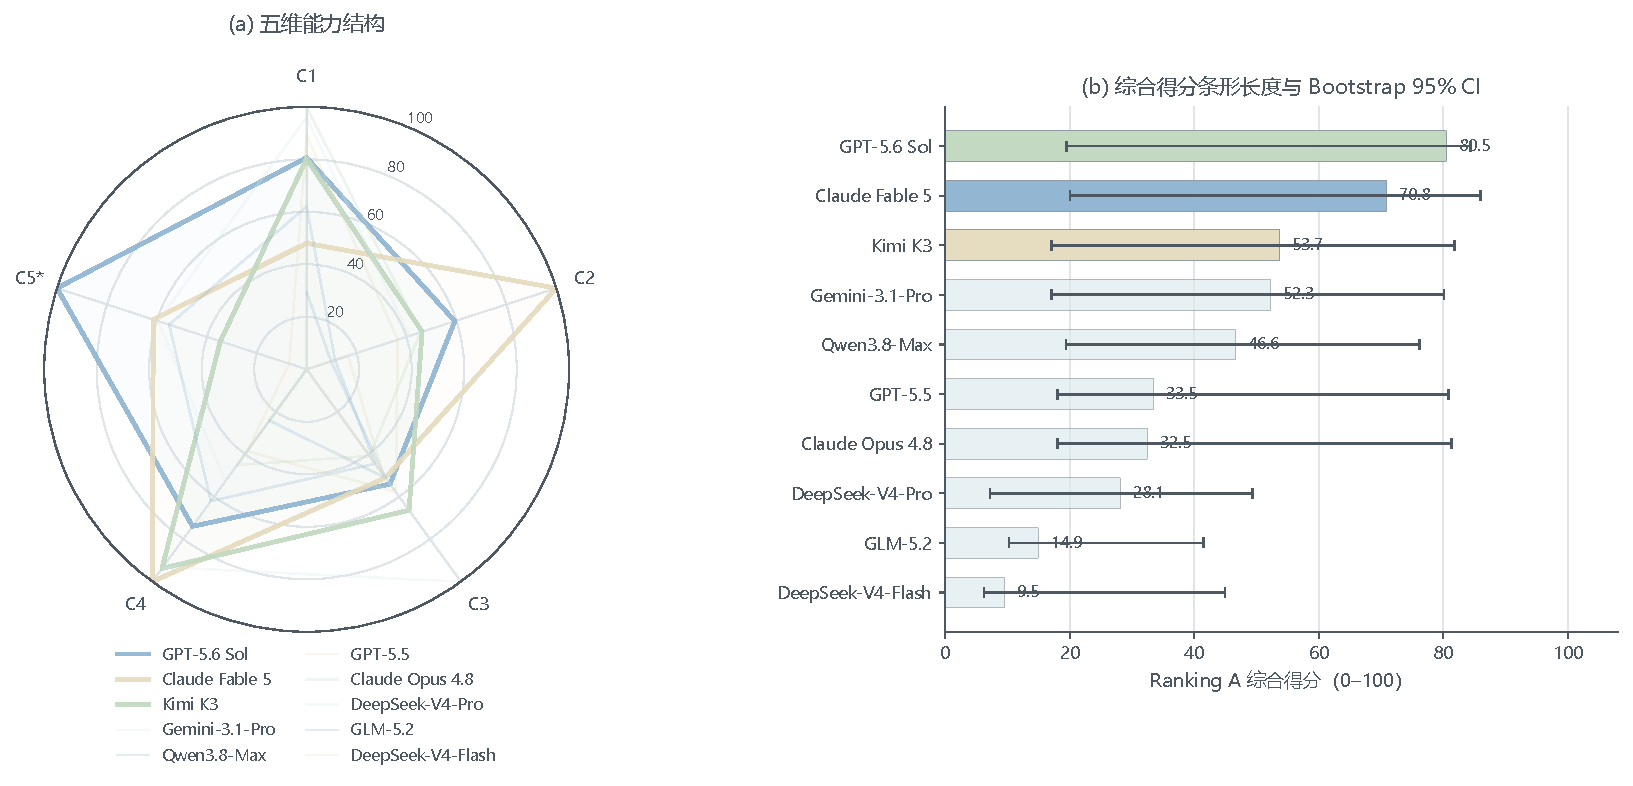
\includegraphics[width=\textwidth]{fig_q1_radar_ranking.pdf}
\caption{各模型五维能力结构与 Ranking A 综合得分。左图展示能力组合，右图为综合得分条形长度及正式 Bootstrap 95\% 置信区间；区间不是市场名次的预测区间。}
\label{fig:q1radar}
\end{figure}

\begin{table}[htbp]
\centering
\caption{Ranking A 主要结果}
\label{tab:q1ranking}
\small
\begin{tabular}{rllrr}
\toprule
排名 & 模型 & 综合得分 & 95\% CI 下界 & 95\% CI 上界\\
\midrule
1 & GPT-5.6 Sol & 80.5 & 19.5 & 84.4\\
2 & Claude Fable 5 & 70.8 & 20.0 & 86.0\\
3 & Kimi K3 & 53.7 & 17.0 & 81.8\\
4 & Gemini-3.1-Pro & 52.3 & 17.1 & 80.1\\
5 & Qwen3.8-Max & 46.6 & 19.4 & 76.2\\
\bottomrule
\end{tabular}
\end{table}

\subsection{不确定性与结构稳健性}

点估计给出的是当前正式数据下的中心评价，而不是绝对稳定的市场名次。图~\ref{fig:q1stability}用 Bootstrap rank 分布展示这一点：小提琴形状反映排名样本的整体分布，箱体表示 IQR，圆点表示 Ranking A 点估计名次。Kimi K3 的 Top-3 经验概率为 \(0.4225\)，排名样本覆盖 \([1,10]\)，说明其第三名位置存在较大的采样不确定性。

\begin{figure}[htbp]
\centering
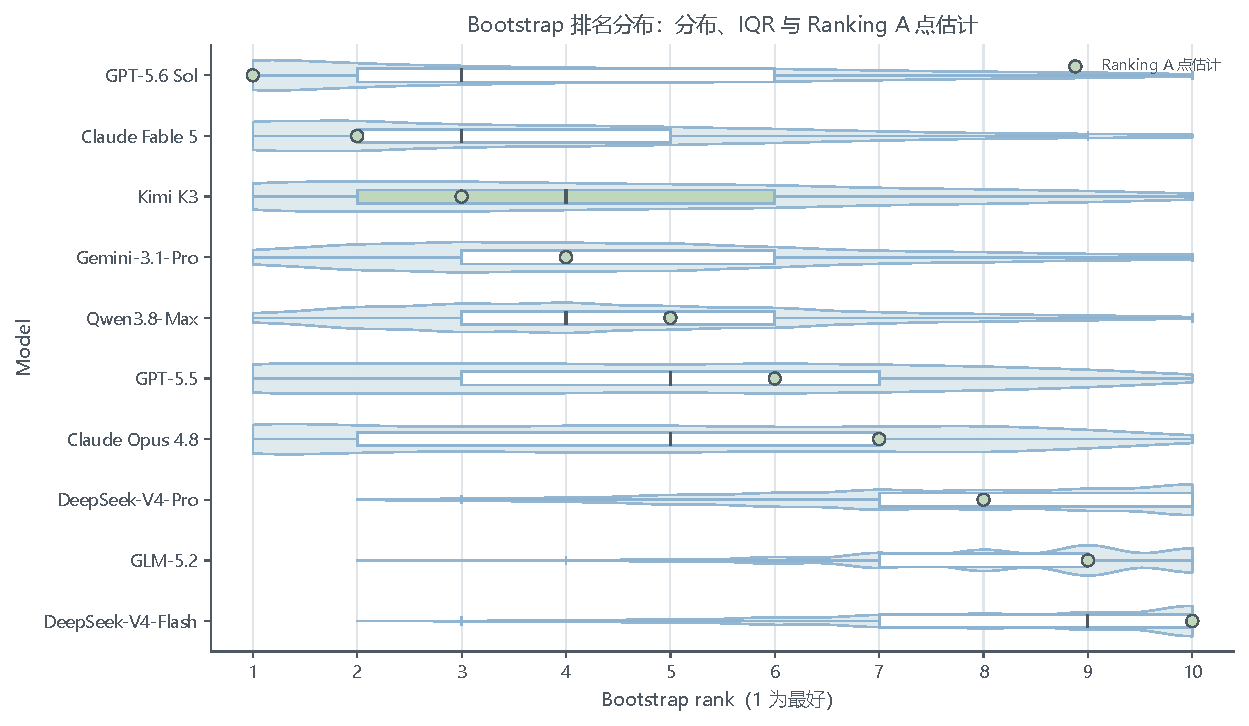
\includegraphics[width=0.86\textwidth]{fig_q1_rank_stability.pdf}
\caption{Ranking A 的 Bootstrap 排名分布。小提琴表示经验分布，箱体表示 IQR，圆点为 Ranking A 点估计排名；排名 1 位于横轴左侧。}
\label{fig:q1stability}
\end{figure}

LOFO 衡量的是对单一 Benchmark 删除的结构鲁棒性。图~\ref{fig:q1robust}显示，在有效情景中，删除单个 Benchmark 后与完整 Ranking A 的秩相关总体较高；删除承担桥接作用的设置时，比较网络可能断开，图中以“network disconnected”直接标记。由此可见，LOFO 说明整体排序结构对单个指标删除具有较强鲁棒性，但不能证明 Bootstrap 下前三名的具体名次稳定。两类检验回答的是不同问题。

\begin{figure}[htbp]
\centering
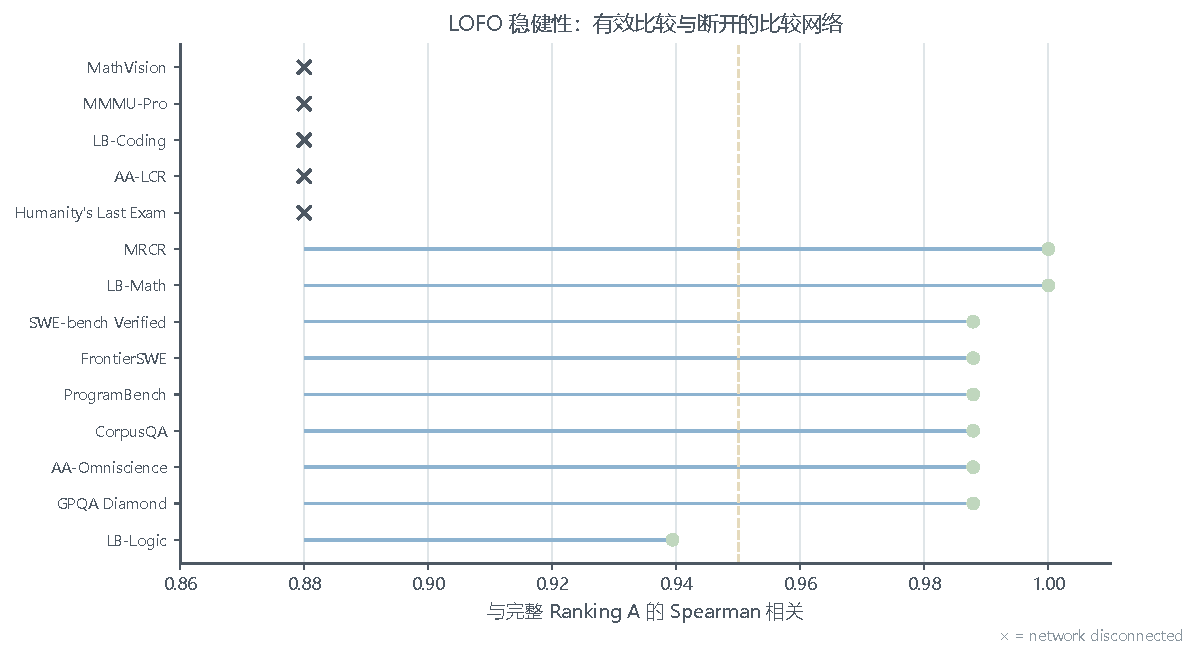
\includegraphics[width=0.78\textwidth]{fig_q1_robustness.pdf}
\caption{LOFO 稳健性：删除单一 Benchmark 后与完整 Ranking A 的秩相关。浅色参考线为 \(\rho=0.95\)，叉号表示比较网络断开。}
\label{fig:q1robust}
\end{figure}



\section{问题二：考虑能力互补的场景效用}
\subsection{为什么综合排名还不能回答场景选择}

问题一得到的是总体能力评价，而题目第二问要求把模型放入具体使用场景。综合排名不能直接表达科研长文本分析、日常通用对话和计算机代码开发对能力组合的差异。若采用线性加权，某一关键能力的不足可以被其他高分能力完全补偿；这与科研和代码任务中短板会限制整体表现的实际特征不符。因此，本问在问题一的能力结果之上，引入场景权重和 CES 聚合。

\subsection{场景需求与 CES 聚合}

设问题一得到的归一化权重先验为 \(\bar w^{Q1}\)。对于场景 \(s\)，在题设约束的可行集合 \(\mathcal C_s\) 上求 KL 最小信息投影：
\[
w^{(s)}=\arg\min_wD_{\mathrm{KL}}(w\Vert\bar w^{Q1}),\qquad
\sum_dw_d=1,\quad w_d\ge0,\quad w\in\mathcal C_s.
\]
正式场景需求为
\[
\begin{aligned}
\text{科研：}\quad &(w_{C1},w_{C2},w_{C3})=(0.3439,0.3250,0.3311),\quad \rho=-0.50,\\
\text{日常：}\quad &(w_{C1},w_{C2},w_{C3},w_{C5})=(0.2417,0.3833,0.1000,0.2750),\quad \rho=0,\\
\text{代码：}\quad &(w_{C1},w_{C4})=(0.3500,0.6500),\quad \rho=-0.40.
\end{aligned}
\]
这些权重不是重新主观打分，而是在问题一客观权重基础上施加场景支持集约束后的最小信息调整。科研场景保留 C1--C3，是因为长文本分析同时需要推理、事实可靠性和上下文处理；代码场景将 C4 置于核心位置，并保留 C1 作为复杂程序任务的推理支撑；日常场景使用更宽的能力集合，以反映通用对话的复合需求。

将各维潜在能力转为同维度内的正值
\[
z_{ij}=\exp(\theta_{ij}-\max_i\theta_{ij}),
\]
并定义
\[
U_i^{(s)}=
\begin{cases}
\left[\displaystyle\sum_{j\in J_s}w_j(s)(z_{ij}+\varepsilon)^{\rho_s}\right]^{1/\rho_s}, & \rho_s\ne0,\\[6pt]
\exp\!\left(\displaystyle\sum_{j\in J_s}w_j(s)\ln(z_{ij}+\varepsilon)\right), & \rho_s=0,
\end{cases}
\qquad \varepsilon=10^{-6}.
\]
当 \(\rho_s<0\) 时，短板会更明显地拖累效用；因此 CES 能够表达“关键能力必须同时达到一定水平”的互补关系。

\begin{figure}[htbp]
\centering
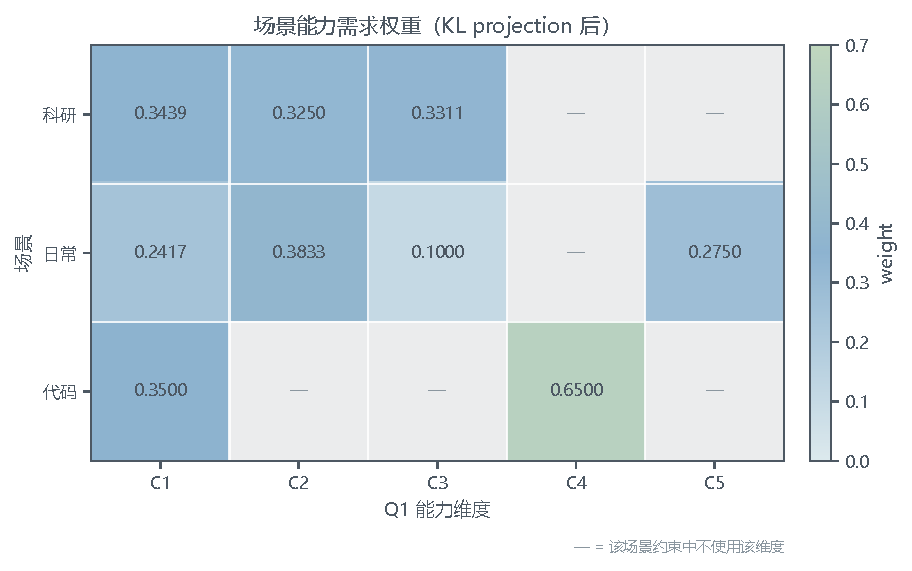
\includegraphics[width=0.78\textwidth]{fig_q2_weight_matrix.pdf}
\caption{三类场景的能力需求权重。行表示场景，列表示 \(C_1\)--\(C_5\)；短横线表示该场景不使用该维度，浅色背景不被解释为权重为零的观测值。}
\label{fig:q2weight}
\end{figure}

\subsection{场景效用结果}

图~\ref{fig:q2utility}将三类场景放在同一矩阵中，但每一列单独进行颜色归一化。单元格数字是正式 CES 效用，颜色只表示对应场景内的相对位置，不用于跨场景绝对比较；边框突出 Top-1 和 Top-3。

\begin{figure}[htbp]
\centering
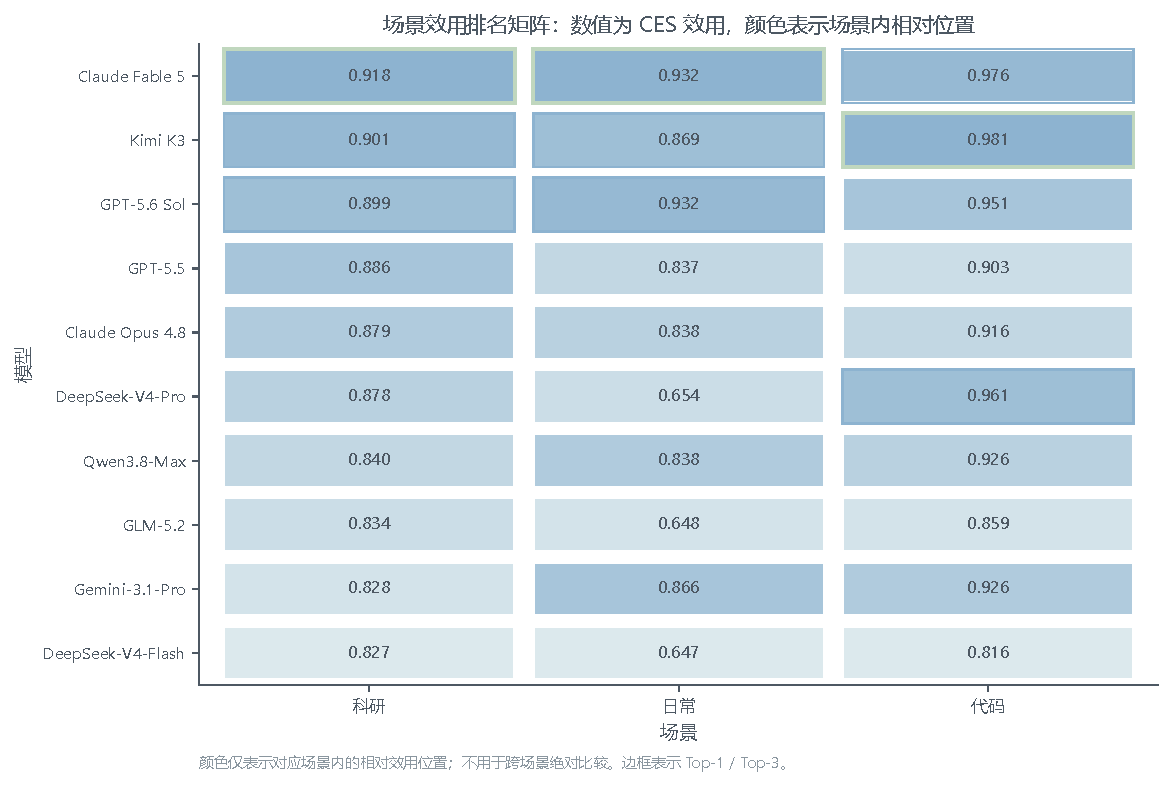
\includegraphics[width=0.92\textwidth]{fig_q2_utility_panels.pdf}
\caption{场景效用排名矩阵。单元格数字为正式 CES 效用，颜色仅表示对应场景内的相对效用位置，不用于科研、日常和代码之间的绝对比较。}
\label{fig:q2utility}
\end{figure}

科研场景中 Claude Fable 5 取得最高效用 \(0.918\)，其次为 Kimi K3 和 GPT-5.6 Sol。其优势并非来自某一单项能力的极端领先，而是 C1--C3 在科研场景权重约束下具有较均衡的组合；当 \(\rho=-0.50\) 时，这种均衡性能够减弱短板惩罚。日常场景中 Claude Fable 5 与 GPT-5.6 Sol 几乎并列第一，说明较高的总体能力和较完整的通用能力组合在该场景中都能转化为效用。代码场景中 Kimi K3 以 \(0.981\) 居首，原因在于 C4 权重达到 \(0.6500\)，其代码工程优势被场景需求直接放大；Claude Fable 5 和 DeepSeek-V4-Pro 分列第二、三位。

\subsection{排名迁移：从总体能力到任务适配}

图~\ref{fig:q2migration}使用 Bump Chart 表示 Ranking A、科研、日常和代码四个阶段的名次迁移。GPT-5.6 Sol 的综合排名为第一，但在科研和代码场景分别调整至第三和第四；Kimi K3 则由综合第三升至代码第一。该变化不是综合模型失稳，而是能力需求映射的结果：综合排名回答“总体上谁更强”，场景排名回答“谁的能力组合更匹配当前任务”。

\begin{figure}[htbp]
\centering
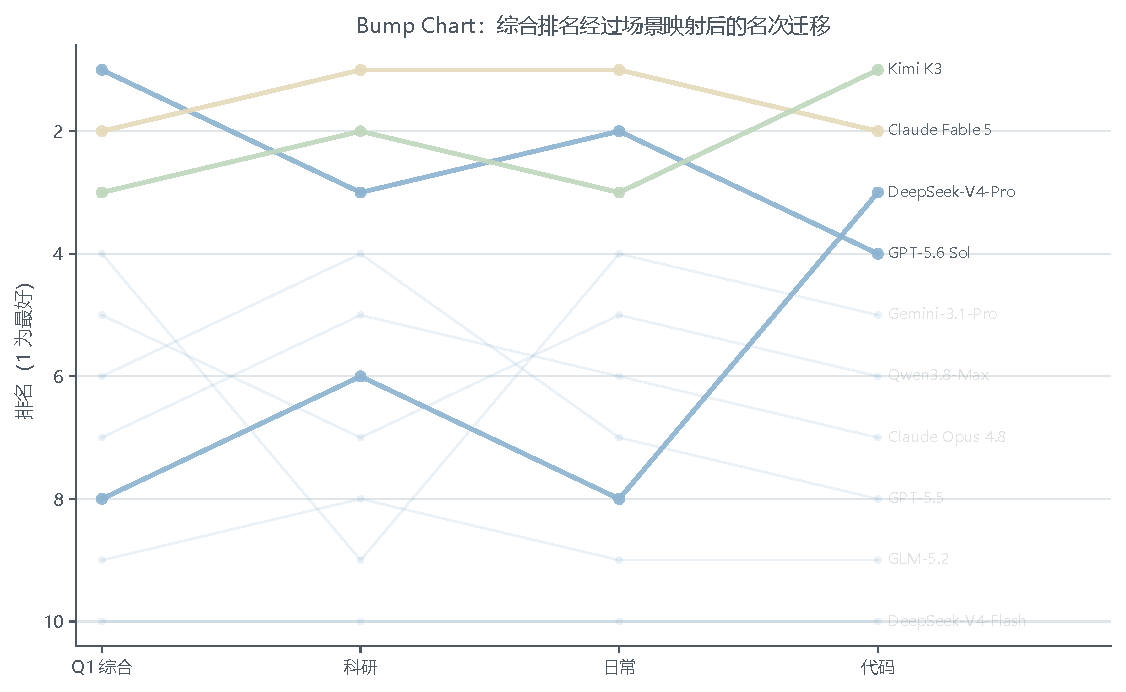
\includegraphics[width=0.90\textwidth]{fig_q2_rank_migration.pdf}
\caption{Bump Chart：Ranking A 到科研、日常和代码场景的排名迁移。重点模型使用高透明度，其余模型保留为低透明度背景线；右端直接标注模型名称。}
\label{fig:q2migration}
\end{figure}

\subsection{CES 排名稳定性}

改变 \(\rho\) 可以检验场景结论是否依赖单一替代弹性点。图~\ref{fig:q2rho}以场景内排名而非效用曲线编码相对位置。测试区间内，科研场景头部模型未出现结构性名次反转；代码场景中 Kimi K3 保持领先。因此，正式结论并非由某一个精确的替代弹性参数点单独驱动。需要强调的是，该检验回答的是参数敏感性，不能替代问题一 Bootstrap 对排名不确定性的检验。

\begin{figure}[htbp]
\centering
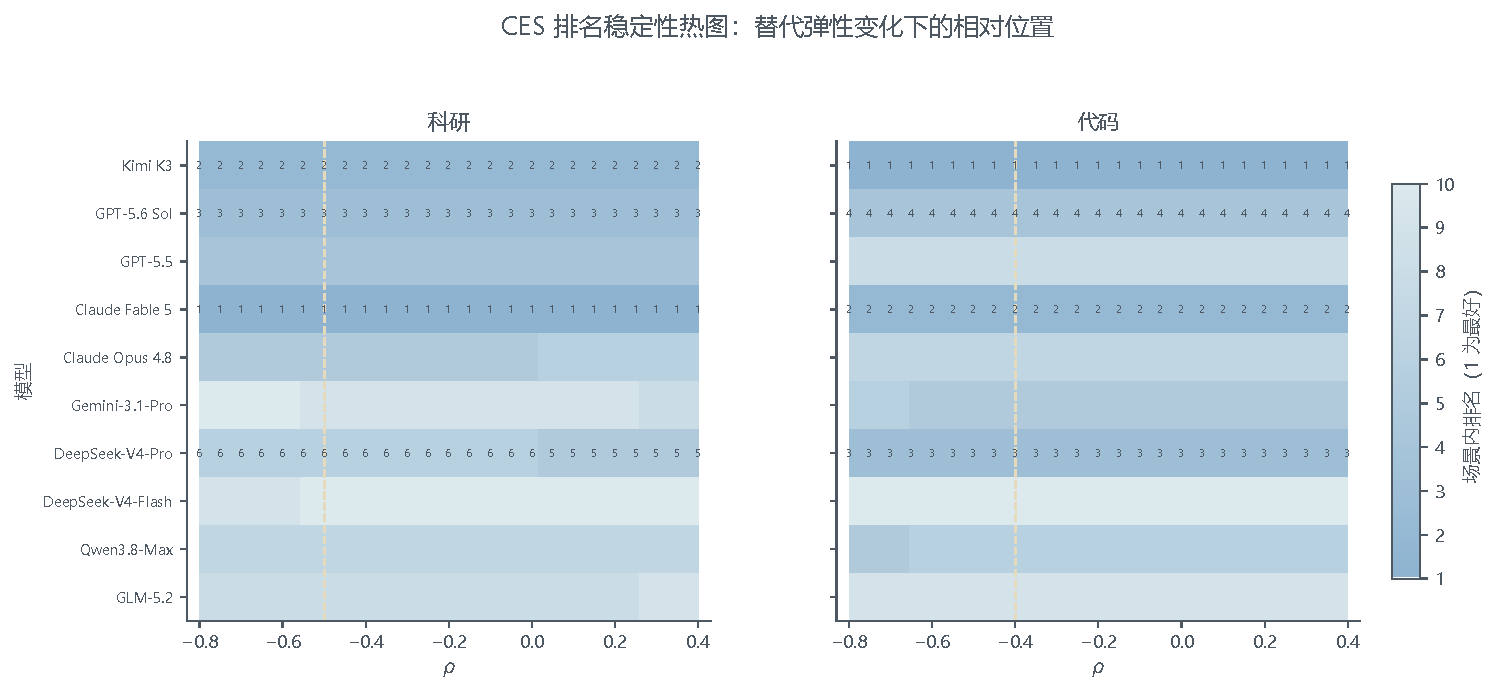
\includegraphics[width=0.90\textwidth]{fig_q2_rho_sensitivity.pdf}
\caption{CES 排名稳定性热图。颜色和格内数字表示场景内排名，竖虚线标出正式 \(\rho\)；颜色不表示跨场景效用的绝对大小。}
\label{fig:q2rho}
\end{figure}


\section{问题三：成本约束下的 Pareto 决策}
\subsection{为什么场景效用还不能决定部署}

问题二给出了模型在不同任务场景中的适配程度，但高效用不等于高性价比，更不等于在预算约束下可执行。输入 Token、输出 Token、调用次数和模型单价共同决定一次标准任务的成本；如果只比较 API 单价，可能忽略工作负载比例带来的成本放大。因此，本问沿用问题二的场景效用，只增加成本维度。

\subsection{工作负载成本}

设模型 \(i\) 的输入、输出单价为 \(p_{\mathrm{in},i}\) 和 \(p_{\mathrm{out},i}\)，场景 \(s\) 的调用次数、计费输入 Token 和计费输出 Token 为 \(N_s,L_{\mathrm{in}}^{(s)},L_{\mathrm{out}}^{(s)}\)。价格单位为 USD/1M billable tokens，则标准任务成本为
\[
C_i^{(s)}
=\frac{N_s}{10^6}
\left[
L_{\mathrm{in}}^{(s)}p_{\mathrm{in},i}
+L_{\mathrm{out}}^{(s)}p_{\mathrm{out},i}
\right].
\]
其中输出 Token 按供应商计费规则计算，包含 reasoning/thinking Token。三类标准工作负载如下：

\begin{table}[htbp]
\centering
\caption{Q3 标准化基准工作负载}
\label{tab:q3workload}
\small
\begin{tabular}{lrrrr}
\toprule
场景 & \(N_s\) & \(L_{\mathrm{in}}\) & \(L_{\mathrm{out}}\) & \(L_{\mathrm{out}}/L_{\mathrm{in}}\)\\
\midrule
科研 & 1 & 16000 & 4000 & 0.25\\
日常 & 1 & 2000 & 1000 & 0.50\\
代码 & 1 & 6000 & 6000 & 1.00\\
\bottomrule
\end{tabular}
\end{table}

代码场景的输出/输入比例为 \(1.00\)，因此输出单价差异会被充分传递到任务成本。图~\ref{fig:q3cost}按总成本从低到高排列成本信息完整且可核验的模型，并将输入、输出两部分分别编码。

\begin{figure}[htbp]
\centering
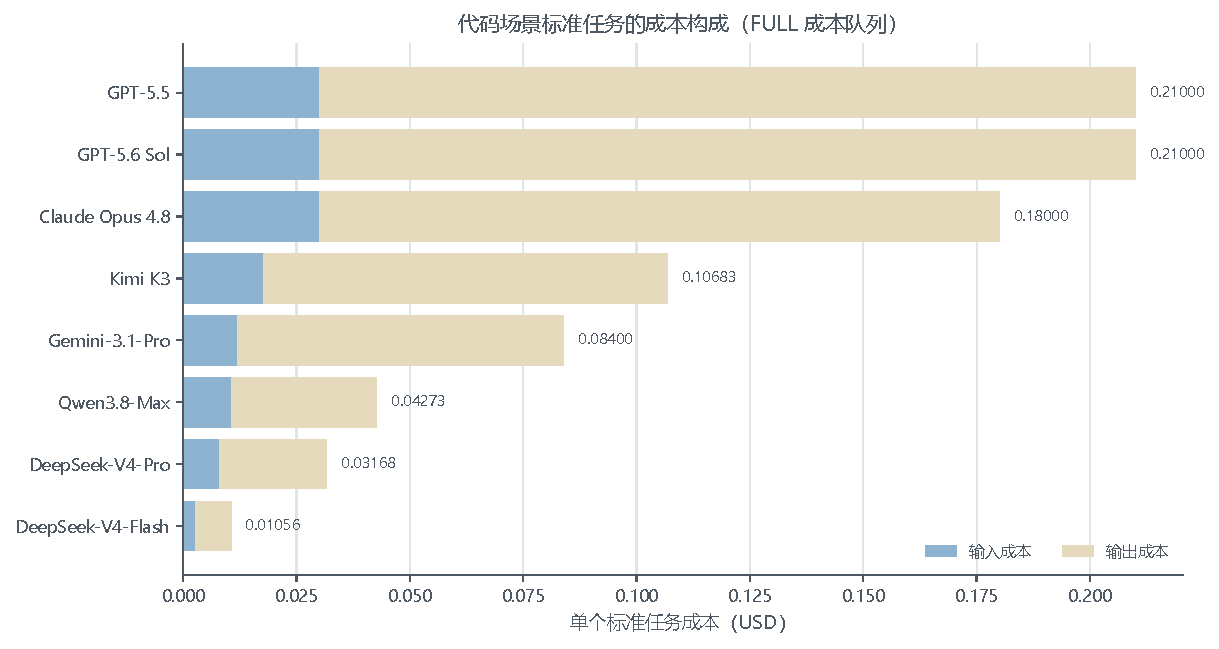
\includegraphics[width=0.84\textwidth]{fig_q3_cost_components.pdf}
\caption{代码场景标准任务的输入/输出成本构成。输入成本为雾蓝，输出成本为奶油米，右端标注总成本。}
\label{fig:q3cost}
\end{figure}

\subsection{成本信息完整性}

严格 Pareto 分析只使用成本信息完整且能够核验的模型集合。Claude Fable 5 的基础 SKU 单价虽然可见，但 max-with-fallback 配置缺少完整的 fallback 目标和二次计费轨迹；GLM-5.2 缺少可复核的公开标准 input/output API 单价。因此二者保留在价格说明中，却不被人工补价，也不被当作零成本模型。该处理使 Q2 的效用优势与 Q3 的部署可决策性保持区分：效用高并不自动意味着成本信息足够完整。

\subsection{Pareto 前沿与场景决策}

在同一场景内，若模型 \(a\) 满足
\[
U_a^{(s)}\ge U_b^{(s)},\qquad C_a^{(s)}\le C_b^{(s)}
\]
且至少一项严格不等，则称 \(a\) 支配 \(b\)。未被任何模型支配的模型构成 Pareto 前沿。图~\ref{fig:q3pareto}保留三个场景的散点表达：绿色点是前沿节点，浅色点是被支配模型，细实线连接按成本排序的前沿。

\begin{figure}[htbp]
\centering
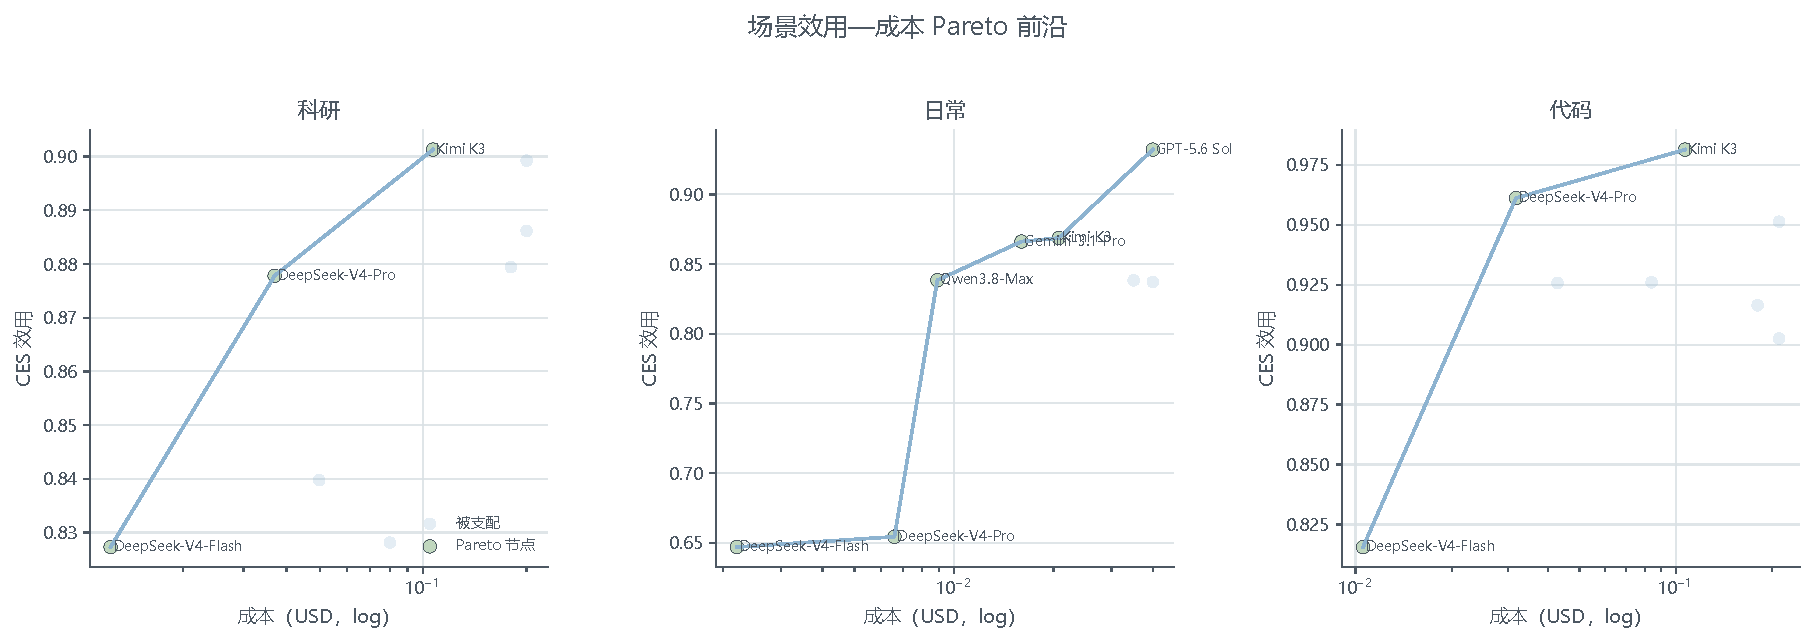
\includegraphics[width=\textwidth]{fig_q3_pareto.pdf}
\caption{科研、日常和代码场景的效用--成本 Pareto 前沿。颜色仅用于区分前沿节点与被支配点，不改变正式效用和成本。}
\label{fig:q3pareto}
\end{figure}

科研场景的前沿依次经过 DeepSeek-V4-Flash、DeepSeek-V4-Pro 和 Kimi K3；日常场景的前沿包含更多节点，并最终到达 GPT-5.6 Sol；代码场景同样由 DeepSeek-V4-Flash、DeepSeek-V4-Pro 和 Kimi K3 构成。以代码任务为例，DeepSeek-V4-Pro 在成本 \(0.03168\) USD 时达到 \(0.9611\) 效用，Kimi K3 在成本 \(0.10683\) USD 时达到 \(0.9813\) 效用。前者代表中等预算下的高效用节点，后者代表更高预算下的效用上限；二者不能用单一“性价比”分数替代。

\subsection{预算约束下的推荐策略}

图~\ref{fig:q3budget}将预算切换点改写为连续的决策区间带。每个区间表示在该预算上限内效用最高的可行节点，分界线直接来自正式预算结果，而不是根据图形外观调整。

\begin{figure}[htbp]
\centering
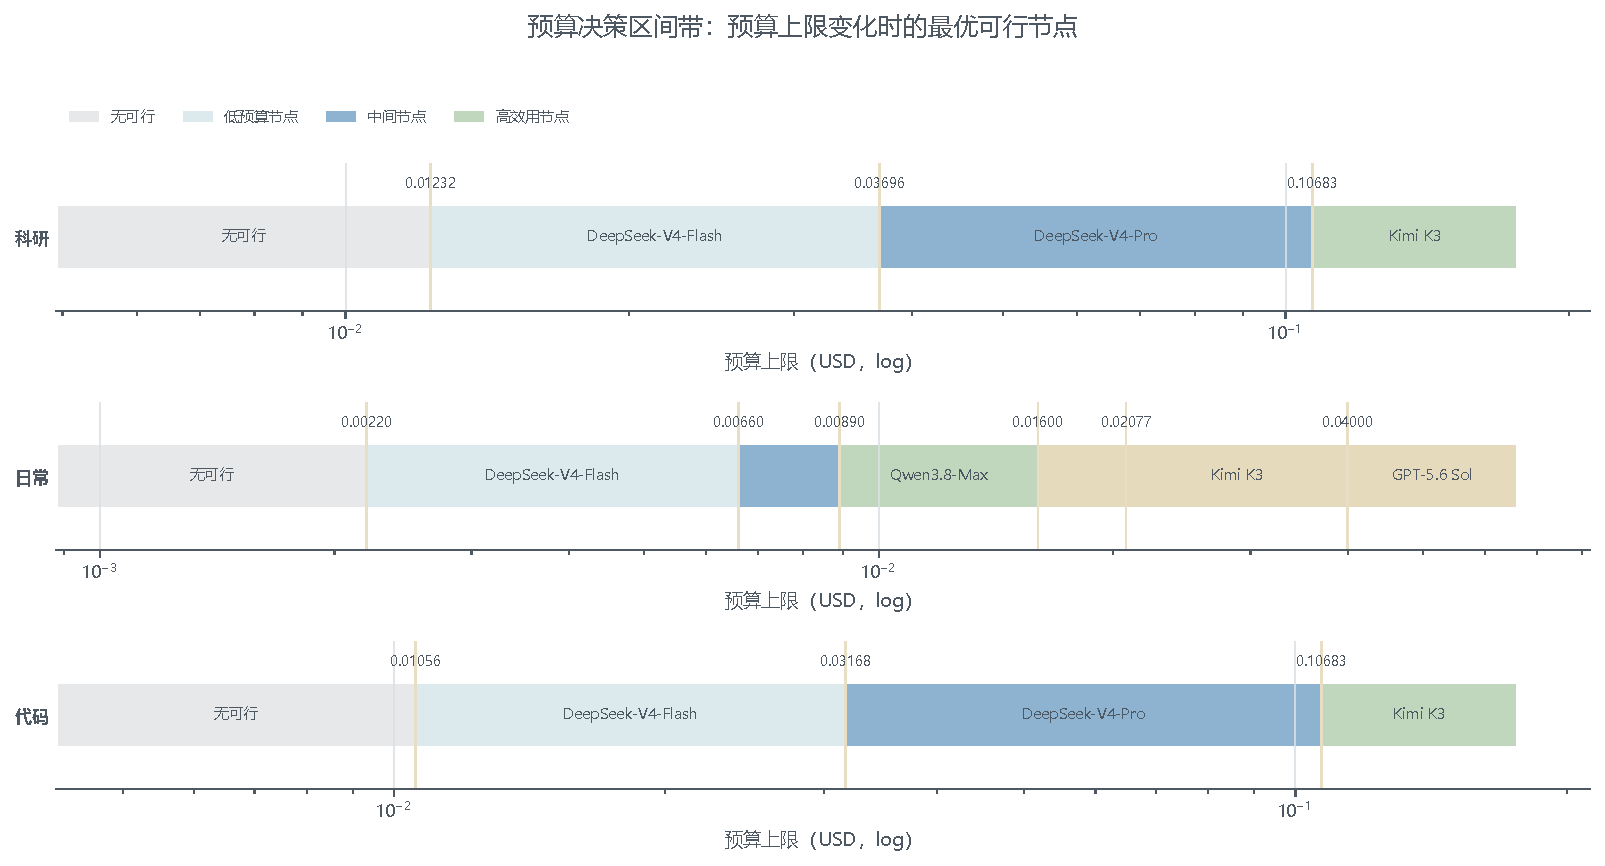
\includegraphics[width=0.92\textwidth]{fig_q3_budget_steps.pdf}
\caption{预算决策区间带。每一行表示一个场景，分界线标注正式预算阈值；区间内文字表示该预算下的最优可行节点。}
\label{fig:q3budget}
\end{figure}

以代码任务为例，当预算低于 \(0.01056\) USD 时，严格成本队列中不存在可行节点；预算达到 \(0.01056\) USD 后，DeepSeek-V4-Flash 首先进入可行集合；预算提高到 \(0.03168\) USD 时，DeepSeek-V4-Pro 以更高效用替代前者；达到 \(0.10683\) USD 后，Kimi K3 成为效用最高的可行方案。科研场景的对应阈值为 \(0.01232\)、\(0.03696\) 和 \(0.10683\) USD；日常场景的切换依次经过 DeepSeek-V4-Flash、DeepSeek-V4-Pro、Qwen3.8-Max、Gemini-3.1-Pro、Kimi K3 和 GPT-5.6 Sol。

因此，Pareto 前沿不是一个静态榜单，而是一组随预算变化的最优候选。Q3 的最终输出不是“价格最低的模型”，而是给定任务场景和预算上限后的可执行推荐。


\section{模型评价与改进}
\subsection{模型优点}

本文模型的优势在于把题目的三层要求分别交给相应的数学工具处理：
\begin{enumerate}[label=(\arabic*),leftmargin=2.5em]
\item 缺失感知评价避免将结构性缺失或未公开成绩误判为低能力；
\item Benchmark Family 平衡抑制测试数量造成的隐性重复赋权；
\item Bradley--Terry 成对比较将不同量纲的公开测试转化为统一的潜在能力尺度；
\item CES 聚合描述任务中的能力互补和短板效应，避免线性加权的完全补偿；
\item 工作负载成本把 API 单价转化为实际任务成本；
\item Pareto 方法保留效用和成本的双重目标，避免人为压缩成一个缺乏解释力的分数；
\item Bootstrap、LOFO、LOSO 和参数敏感性从不同角度检验结论对数据与设定变化的响应。
\end{enumerate}

\subsection{局限与改进方向}

第一，公开 Benchmark 是横截面信息，不能完全替代统一实验环境，模型版本和测试协议变化也可能影响横向比较。第二，Bradley--Terry 能力估计依赖可观测比较网络；当桥接设置缺失时，部分维度可能出现网络断开或结构依赖。第三，C5 的有效模型范围较小，相关结论应与适用性审计一并解释。第四，Q2 不确定性传播采用正式接口给出的独立正态近似场景样本，而不是带完整协方差的联合 Q1 Bootstrap。第五，Q3 使用标准化工作负载，不能替代特定用户的真实 Token 分布；价格也可能随时间变化。最后，成本信息不完整的模型无法进入严格 Pareto，这体现了部署决策的可核验性要求，也限制了效用与成本的直接覆盖范围。

后续可在统一评测协议下补充联合 Bootstrap 协方差、时间序列价格、真实 Token 负载、延迟和吞吐等部署指标，并在保留 Pareto 结构的前提下扩展多目标决策。


\section{结论}
本文针对题目提出的模型综合评价、场景选择与成本约束决策问题，构建了由基础能力、场景适配和预算约束组成的递进模型。

问题一在 \(164/210=78.1\%\) 的有效公开观测下，先区分普通缺失与结构性缺失，再通过缺失感知相关性、Family 平衡成对比较和正则化 Bradley--Terry 得到五维能力结构。Ranking A 的点估计中，GPT-5.6 Sol、Claude Fable 5 和 Kimi K3 位列前三；但 Bootstrap 区间较宽，Kimi K3 的 Top-3 经验概率为 \(0.4225\)，因此该排序应理解为正式数据下的中心评价，而不是绝对稳定的市场名次。

问题二说明综合能力并不等于任务适配。科研场景中 Claude Fable 5 居首，原因是 C1--C3 的能力组合较均衡，在负替代弹性下短板惩罚较小；代码场景中 Kimi K3 居首，原因是代码工程能力 C4 在场景权重中占主导；GPT-5.6 Sol 虽然综合排名第一，但在科研和代码场景中的位置发生变化。这说明模型选择必须经过能力需求映射，而不能停留在总体榜单。

问题三进一步将场景效用与工作负载成本结合。代码场景的预算决策依次经过 DeepSeek-V4-Flash、DeepSeek-V4-Pro 和 Kimi K3，切换阈值为 \(0.01056\)、\(0.03168\) 和 \(0.10683\) USD。效用优势只有在成本信息完整且预算允许时，才能转化为可执行的部署方案；因此，效用高但成本不可核验的模型不应被强行纳入严格 Pareto。

综上，题目的最终决策逻辑为
\[
\boxed{
\text{基础能力识别}
\longrightarrow
\text{场景适配}
\longrightarrow
\text{预算约束下的决策}
}.
\]
若关注综合能力，应参考 Ranking A 的中心评价并同时查看不确定性；若属于科研任务，应优先比较科研场景中的效用与短板结构；若属于代码任务，应重点考察 C4 主导下的场景效用；若成本敏感，则沿相应场景的 Pareto 前沿选择；随着预算提高，再根据预算决策区间带切换到更高效用节点。由此，不存在脱离任务需求与预算约束的绝对最优模型。


\begin{thebibliography}{99}

\bibitem{BradleyTerry1952}
Bradley R A, Terry M E. Rank analysis of incomplete block designs: I. The method of paired comparisons[J]. \textit{Biometrika}, 1952, 39(3--4): 324--345.

\bibitem{Spearman1904}
Spearman C. The proof and measurement of association between two things[J]. \textit{The American Journal of Psychology}, 1904, 15(1): 72--101.

\bibitem{ArrowEtAl1961}
Arrow K J, Chenery H B, Minhas B S, Solow R M. Capital-labor substitution and economic efficiency[J]. \textit{The Review of Economics and Statistics}, 1961, 43(3): 225--250.

\bibitem{Pareto1906}
Pareto V. \textit{Manuale di economia politica}[M]. Milano: Società Editrice Libraria, 1906.

\bibitem{GPQA}
Rein D, Hou B L, Stickland A C, et al. GPQA: A graduate-level Google-proof Q\&A benchmark[EB/OL]. Official benchmark repository: \url{https://github.com/idavidrein/gpqa}.

\bibitem{LiveBench}
LiveBench. LiveBench official benchmark site[EB/OL]. \url{https://livebench.ai/}.

\bibitem{HLE}
Center for AI Safety. Humanity's Last Exam official repository[EB/OL]. \url{https://github.com/centerforaisafety/hle}.

\bibitem{MMMUPro}
Yue X, Ni Y, Zhang K, et al. MMMU-Pro official benchmark repository[EB/OL]. \url{https://github.com/MMMU-Benchmark/MMMU}.

\bibitem{MathVision}
MathVision official benchmark repository[EB/OL]. \url{https://github.com/mathvision-cuhk/MathVision}.

\bibitem{OpenAIOfficial}
OpenAI. GPT-5.5 and GPT-5.6 Sol model documentation and API pricing[EB/OL]. Snapshot recorded in the frozen Q3 pricing audit on 2026-08-17. \url{https://developers.openai.com/api/docs/models/gpt-5.6-sol}.

\bibitem{AnthropicOfficial}
Anthropic. Claude model documentation and API pricing[EB/OL]. Snapshot recorded in the frozen Q3 pricing audit on 2026-08-17. \url{https://docs.anthropic.com/en/docs/about-claude/pricing}.

\bibitem{GoogleOfficial}
Google DeepMind. Gemini API model documentation and pricing[EB/OL]. Snapshot recorded in the frozen Q3 pricing audit on 2026-08-17. \url{https://ai.google.dev/gemini-api/docs/pricing}.

\bibitem{DeepSeekOfficial}
DeepSeek. API model documentation and pricing[EB/OL]. Snapshot recorded in the frozen Q3 pricing audit on 2026-08-17. \url{https://api-docs.deepseek.com/quick_start/pricing}.

\bibitem{KimiOfficial}
Moonshot AI. Kimi K3 official model documentation and pricing[EB/OL]. Snapshot recorded in the frozen Q3 pricing audit on 2026-08-17. \url{https://platform.kimi.com/docs/pricing/chat-k3.md}.

\bibitem{QwenOfficial}
Alibaba Cloud. Qwen model studio pricing documentation[EB/OL]. Snapshot recorded in the frozen Q3 pricing audit on 2026-08-17. \url{https://help.aliyun.com/zh/model-studio/model-pricing}.

\bibitem{GLMOfficial}
Zhipu AI. GLM-5.2 model documentation[EB/OL]. Snapshot recorded in the frozen Q3 pricing audit on 2026-08-17. \url{https://docs.bigmodel.cn/cn/guide/models/text/glm-5.2.md}.

\end{thebibliography}


\appendix
\section{补充稳健性与价格快照}

\subsection{完整排名概率矩阵}

正文图 5 使用排名分布表达 Bootstrap 不确定性；完整的 \(P(\mathrm{rank}=r)\) 矩阵保留在附录，以便复核每个模型在每个名次上的经验概率。

\begin{figure}[htbp]
\centering
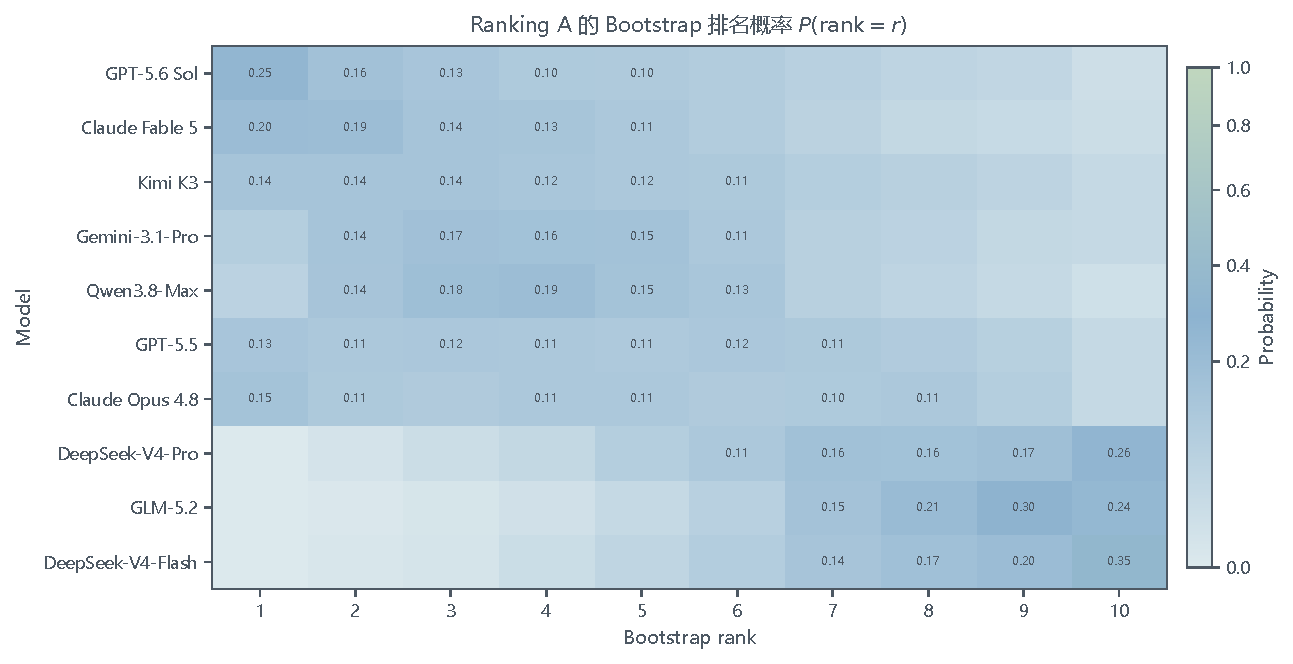
\includegraphics[width=0.86\textwidth]{appendix_archive/fig_q1_rank_stability_v2.pdf}
\caption{Ranking A 的完整 Bootstrap 排名概率矩阵。该图为正文旧版的附录保留，不作为正文主结论图。}
\label{fig:appendix_rank_probability}
\end{figure}

\subsection{其他补充图形}

旧版 CES 效用曲线、原始预算阶梯图和完整场景效用点线图均保留在论文工作区的附录图形目录中，其数值与正式结果一致，但不再承担正文的主要解释任务。正文优先保留能够区分数据结构、能力评价、不确定性、场景迁移、参数稳健性、成本、Pareto 和预算决策的信息图形。

\subsection{LOSO 稳健性}
LOSO 结果直接读取 Q1 正式输出。有效比较保留共同模型数、与完整 Ranking A 的 Spearman 相关、Kimi 的其他排名和前三重叠数；比较网络断开时以 $\times$ 标记，不将其填充为数值。

\begin{table}[htbp]
\centering
\caption{LOSO 场景/来源删除审计。数据源：\texttt{outputs/q1\_v1.2/tables/table\_q1\_v12\_loso.xlsx}，sheet \texttt{Scenario\_Summary}。}
\label{tab:loso}
\small
\begin{tabularx}{\textwidth}{lrrrrl}
\toprule
删除对象 & Common-N & Spearman & Kimi 其他排名 & Top-3 重叠 & 状态\\
\midrule
LiveBench & $\times$ & -- & -- & -- & -- \\
Artificial Analysis & $\times$ & -- & -- & -- & -- \\
Kimi official/technical comparison & $\times$ & -- & -- & -- & -- \\
DeepSeek technical report & 10 & 1.000 & 3 & 3 & OK \\
OpenRouter & 10 & 0.988 & 3 & 3 & OK \\
\bottomrule
\end{tabularx}
\end{table}

\subsection{等权敏感性}
将 Q1 综合权重替换为五维等权后，Ranking A 前三模型及其顺序保持不变；完整十模型的名次变化见表~\ref{tab:equalweight}。该表只报告正式等权敏感性输出，不重新估计任何分数。

\begin{table}[htbp]
\centering
\caption{等权敏感性的逐模型比较。}
\label{tab:equalweight}
\small
\begin{tabularx}{\textwidth}{rXrrrr}
\toprule
完整排名 & 模型 & 等权排名 & 名次变化 & 原得分 & 等权得分\\
\midrule
1 & GPT-5.6 Sol & 1 & 0 & 80.5 & 73.6 \\
2 & Claude Fable 5 & 2 & 0 & 70.8 & 72.1 \\
3 & Kimi K3 & 3 & 0 & 53.7 & 64.2 \\
4 & Gemini-3.1-Pro & 4 & 0 & 52.3 & 49.8 \\
5 & Qwen3.8-Max & 5 & 0 & 46.6 & 47.0 \\
6 & GPT-5.5 & 8 & +2 & 33.5 & 45.7 \\
7 & Claude Opus 4.8 & 6 & -1 & 32.5 & 46.3 \\
8 & DeepSeek-V4-Pro & 7 & -1 & 28.1 & 46.1 \\
9 & GLM-5.2 & 9 & 0 & 14.9 & 22.9 \\
10 & DeepSeek-V4-Flash & 10 & 0 & 9.5 & 13.2 \\
\bottomrule
\end{tabularx}
\end{table}

\subsection{动态价格记录}
价格只用于 Q3 成本审计，冻结快照日期、API SKU、评测配置和供应商官方来源均保留在表~\ref{tab:pricing_snapshot}。其中 \texttt{SPECIAL\_CASE} 和缺失价格不会被视为零成本，也不进入严格 FULL 主 Pareto。

\begin{table}[htbp]
\centering
\caption{Q3 动态价格快照与 SKU/configuration 记录。数据源：\texttt{q3/frozen/v1.0/model\_pricing.csv}；price\_date 为冻结/快照日期。}
\label{tab:pricing_snapshot}
\scriptsize
\begin{tabularx}{\textwidth}{p{3.0cm}p{1.6cm}p{6.0cm}X}
\toprule
模型 & 快照日期 & SKU / exact configuration & 官方来源\\
\midrule
Kimi K3 (max reasoning) & 2026-08-17 & kimi-k3 reasoning\_effort=max / kimi-k3 & \href{https://platform.kimi.com/docs/pricing/chat-k3.md}{official} \\
GPT-5.6 Sol (max) & 2026-08-17 & gpt-5.6-sol reasoning.effort=max / gpt-5.6-sol & \href{https://developers.openai.com/api/docs/models/gpt-5.6-sol}{official} \\
GPT-5.5 (xhigh) & 2026-08-17 & gpt-5.5 reasoning.effort=xhigh / gpt-5.5 & \href{https://developers.openai.com/api/docs/models/gpt-5.5}{official} \\
Claude Fable 5 (max, with fallback) & 2026-08-17 & claude-fable-5 base model with benchmark fallback / claude-fable-5 & \href{https://docs.anthropic.com/en/docs/about-claude/pricing}{official} \\
Claude Opus 4.8 (max) & 2026-08-17 & claude-opus-4-8 effort=max / claude-opus-4-8 & \href{https://docs.anthropic.com/en/docs/about-claude/pricing}{official} \\
Gemini-3.1-Pro (High) & 2026-08-17 & gemini-3.1-pro-preview thinking\_level=high / gemini-3.1-pro-preview & \href{https://ai.google.dev/gemini-api/docs/pricing}{official} \\
DeepSeek-V4-Pro Max & 2026-08-17 & DeepSeek-V4-Pro-0813 thinking mode / deepseek-v4-pro & \href{https://api-docs.deepseek.com/quick_start/pricing}{official} \\
DeepSeek-V4-Flash Max & 2026-08-17 & DeepSeek-V4-Flash-0731 thinking mode / deepseek-v4-flash & \href{https://api-docs.deepseek.com/quick_start/pricing}{official} \\
Qwen3.8-Max & 2026-08-17 & qwen3.8-max thinking or non-thinking mode / qwen3.8-max & \href{https://help.aliyun.com/zh/model-studio/model-pricing}{official} \\
GLM-5.2 (max) & 2026-08-17 & glm-5.2 reasoning\_effort=max / glm-5.2 & \href{https://docs.bigmodel.cn/cn/guide/models/text/glm-5.2.md}{official} \\
\bottomrule
\end{tabularx}
\end{table}


\end{document}
